\section{Unfolding and Folding}

% unfolding and folding
The extensions of Petri nets that CPNs bring in the form of data
types, a programming language, and modules add practical modeling
power to Petri nets making it feasible to create models of complex
real systems. PTNs extended with \concept{inhibitor arcs} allowing a
test for zero tokens on a place can already simulate Turing machines
and hence the CPN extensions do not add expressive power from a
theoretical perspective. Furterhmore, any hierarchical CPN model can
be \concept{unfolded} to a non-hierarchical CPN model which in turn
can be unfolded to a behaviorally equivalent PTN model. In the other
direction, any PTN model also including inhibitor arcs can be
\concept{folded} into a CPN model with a single module consisting of a
single place and a single transition. In practice such a folding is
not interesting, because the arc expressions will be extremely complex
and non-interpretable for a human being. However, the fact that the
unfolding and folding exist shows that hierarchical CPNs have the same
behavioral properties as basic Petri nets, and hence constitutes a
solid model for concurrency, conflict, synchronization and resource
sharing.

%Anything which can be programming in Java can (in theory) also be
%programmed in assembler code. It is just much more time-consuming and
%much more error-prone. 

%Analogously it can be proved (quite easily) that each hierarchical CPN
%can be unfolded to a (much larger) basic Petri net (Place Transition
%Net) with exactly the same dynamic behavior.

% illustrate place and transition unfolding

\begin{figure}[]
\centering
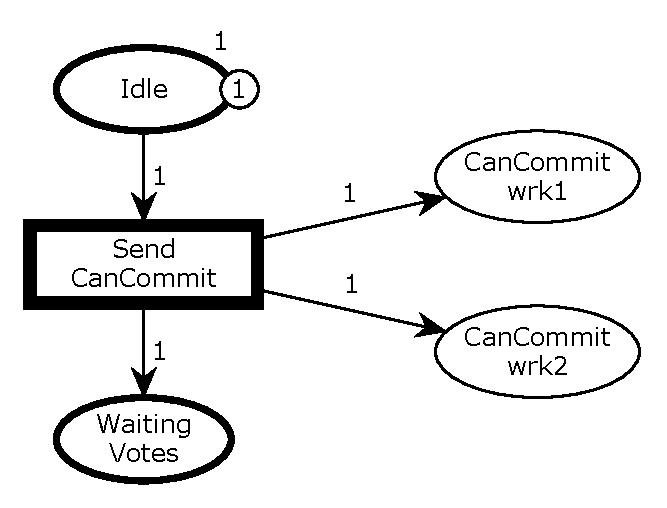
\includegraphics[scale=.43]{figures/PTSendCanCommit.eps}
\caption{PTN representation of the CPN in Fig.~\ref{fig:sendcancommit}.}
\label{fig:sendcancommitunfold}
\end{figure}

\begin{figure*}[t!!!!!]
\centering
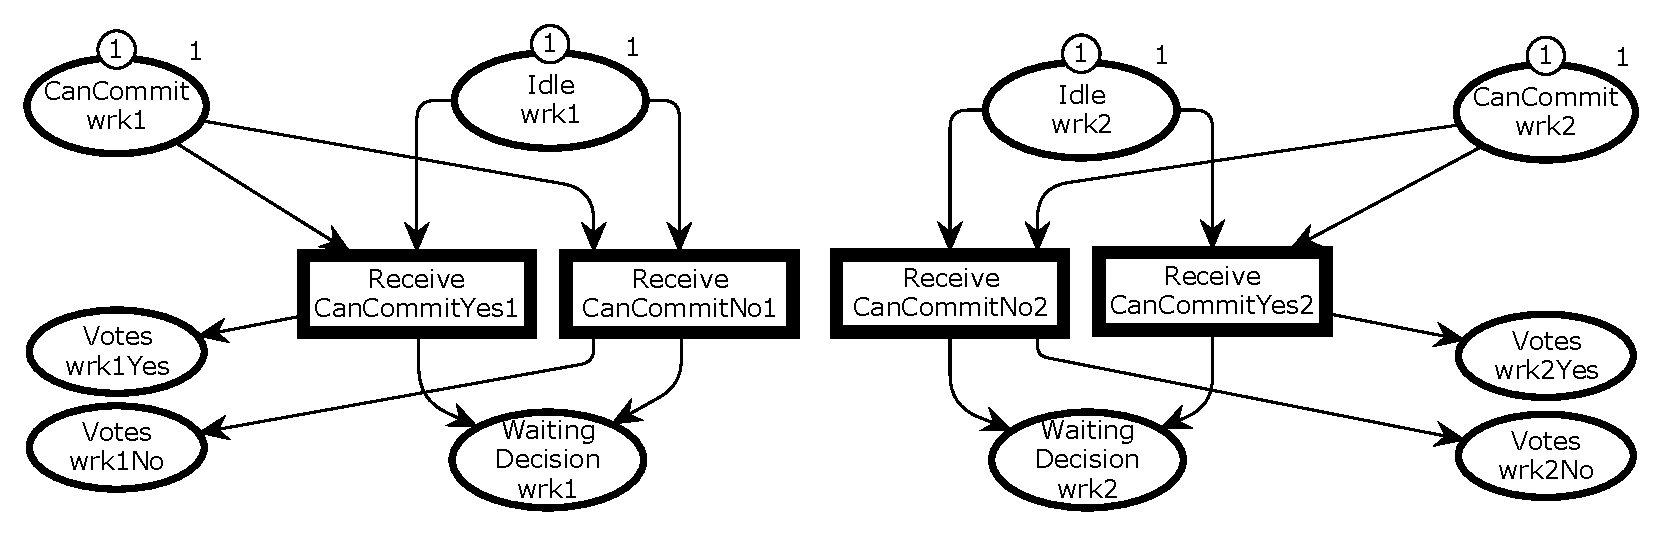
\includegraphics[scale=.43]{figures/PTReceiveCanCommitBoth.eps}
\caption{PTN representation of the CPN in Fig.~\ref{fig:receivecancommit}.}
\label{fig:receivecancommitunfold}
\end{figure*}


The unfolding of a hierarchical CPN to a non-hierarchical CPN consists
of recursively replacing each substitution transition with its
associated submodule such that associated port and socket places are
merged into a single place. The unfolding of a non-hierarchical CPN to
a PTN consists of unfolding each CPN place to a PTN place for each
color in the color set of the CPN place, and unfolding each CPN
transition to a PTN transition for each possible binding of the CPN
transition.  To illustrate the unfolding consider the subnet in
Fig.~\ref{fig:sendcancommit}. To represent this CPN subnet as a PTN,
the CPN place \figitem{CanCommit} needs to be unfolded to two PTN
places corresponding to \smlcode{wrk(1)} and \smlcode{wrk(2)}. The
places \figitem{Idle} and \figitem{WaitingVotes} do not need to be
unfolded as the \smlcode{Unit} color set contains only a single
value. The equivalent PTN is shown in
Fig.~\ref{fig:sendcancommitunfold}. It can be seen that the arc
expressions are replaced by arc weights, and that the initial marking
is replaced by a single token initially in \figitem{Idle}.

To show the unfolding of a CPN transition consider the CPN subnet
shown in Fig.~\ref{fig:receivecancommit}. To represent this subnet as
a PTN, we need to unfold the places as explained in the previous
paragraph and in addition unfold the transition
\figitem{ReceiveCanCommit} to a PTN transition for each of the four
binding elements listed in
Fig.~\ref{fig:bindings}. Figure~\ref{fig:receivecancommitunfold} shows
the equivalent PTN (arc weights have been omittted as all are 1).

% Similarly, no unfolding of the \figitem{SendCanCommit}
%transition is required in this case since the transition does not have
%any variables. 

% illustrate transition unfolding

% It can be seen that we essentially
%need a copy of the CPN fragment for each worker in the system.

Above we have shown how to unfold two CPN subnets into PTN subnets.
For larger color sets the unfolding yields an explosion in size, since
we have a PTN place for each color of a CPN place and a PTN transition
for each binding of a CPN transition. For our CPN model we just need
to change the symbolic constant \smlcode{W}
(cf. Fig.~\ref{fig:coloursets}) to configure the model to handle,
e.g., five workers. With basic Petri nets we need to add places,
transitions, and arcs and hence change the net structure. This shows
that CPNs (in contrast to basic Petri nets) provides a means for
easily creating parameterizable models and also enable more compact
modeling.\rdc{With CPN it is possible to have many color sets and hence we
can use one color set for the coordinator, a second for the workers, a
third for Yes/No votes and a fourth for Abort/Commit decisions. With
PrT nets only a single set of token colors is allowed (or Cartesian
products thereof) and hence we need to encode the identity of workers,
Yes/No votes and Abort/Commit decisions into this single set of token
colors.}

\ignore{
The unfolding above demonstrates that Petri nets in their basic form
do not provide a way to easily scale the model according to some
system parameter (in this case the number of workers). It is necessary
to have a subnet for each worker (even though they behave in exactly
the same way). With PrT nets and CPNs we can use tokens with color
\smlcode{wrk(1)} to model the state of the first worker, tokens with
the color \smlcode{wrk(2)} to model the state of the second worker,
and so on. This means that we for \smlcode{W} workers can have a
single \figitem{Idle} place, which may contain tokens of \smlcode{W}
different colors -- instead of having a separate \smlcode{Idle} place
for each of the \smlcode{W} workers. In particular, in the CPN model
where we just need to change the symbolic constant \smlcode{W} (see
Fig.~\ref{fig:coloursets}) to configure the model to handle, e.g.,
five workers whereas with basic Petri nets we need to add places,
transitions, and arcs and hence change the net structure in order to
increase the number of workers.  This shows that CPNs provides a means
for easily creating parameterizable models and also that it enables
more compact modeling as we only need a single instance of the
\figitem{CanCommit} place in order to accommodate any finite number of
workers. Comparing CPN and PrT nets. With CPN it is possible to have
many color sets and hence we can use a number of different color sets
(e.g. one color set for the coordinator, a second for the workers, a
third for yes/no votes and a fourth for abort/commit decisions). With
PrT nets only one set of token colors are allowed (or Cartesian
product thereof) and hence with PrT nets we could have had to
represent the identity workers, yes/No votes and abort/commit
decisions by colors based on this single set of token colors.
}
